% The topical focus of the session is single and multi-robot systems
% that use network-based, distributed implementations of their
% sensing and control.
% 
% Topics of interest for the session include, but are not limited to, the
% following themes:
% 
% - decentralised control (e.g. distributed behaviour-based systems).
% - distributed object-oriented and multi-agent systems/architectures
% - sensor fusion (e.g. distributed, decentralised, algorithms)
% - modular and reconfigurable robot systems
% - communications networks and protocols for multi-robot systems
% - mutli-robot coordination (dual-robot transport, cooperative robotics)
% - and expiermental development and characterization of these topics
%   in fielded systems

%
% Reviewer's comments:
% 
% It was not clear to this reviewer how the approach outlined in the paper
% would extend to complex robotic systems whose design involves a range
% of hierarchically organized hardware and software functions and devices,
% as opposed to the simple robotic mechanisms that appear to be the current
% research focus.   Suggest a discussion of the relevance of the approach
% to more complex robotic systems.
%


% length limit: 6 pages (A4)

% $Id: icar03-player.tex,v 1.42 2003/07/15 18:26:14 gerkey Exp $

\documentclass[a4paper]{ICAR2003}
\usepackage{times}
\usepackage{epsfig}
\usepackage[a4]{pubref}
\pubref{Proceedings of the International Conference on Advanced Robotics
(ICAR 2003)} {pages 317-323, Coimbra, Portugal, June 30 - July 3, 2003.}

\pagestyle{empty}
\thispagestyle{empty}

\begin{document} 

\title{The Player/Stage Project:\\ Tools for Multi-Robot and Distributed
Sensor Systems}
\author{\begin{tabular}{ccc}
\bf Brian P. Gerkey & \bf Richard T. Vaughan & \bf Andrew Howard \\
Robotics Research Lab & Information Sciences Lab & Robotics Research Lab\\
University of Southern California & HRL Labs & University of Southern
California\\
Los Angeles, California & Malibu, California & Los Angeles, California\\
\tt \small gerkey@robotics.usc.edu & \tt \small vaughan@hrl.com &
\tt \small ahoward@robotics.usc.edu
\end{tabular}}
\date{}


\maketitle
\thispagestyle{empty}

\begin{Abstract}
This paper describes the {\em Player/Stage} software tools applied
to multi-robot, distributed-robot and sensor network systems.  {\it
Player} is a robot device server that provides network transparent
robot control. Player seeks to constrain controller design as little
as possible; it is device independent, non-locking and language- and
style-neutral. {\it Stage} is a lightweight, highly configurable robot
simulator that supports large populations.  Player/Stage is a community
Free Software project.  Current usage of Player and Stage is reviewed, and
some interesting research opportunities opened up by this infrastructure
are identified.
\end{Abstract} 

\section{Introduction}
Programming robots is complicated and time-consuming. Working with
multiple and distributed robot systems is further complicated by (i)
more robots and (ii) the difficulties of network programming.  The {\em
Player/Stage Project} provides Open Source tools that simplify controller
development, particularly for multiple-robot, distributed-robot, and
sensor network systems (hereafter referred to collectively as Multi-Robot
Systems (MRS)).

This paper provides an overview of the Player/Stage tools and their
application to MRS. We describe the tools and review published MRS
work using Player/Stage, as well as describe some of the under-explored
research opportunities opened up by this infrastructure.

The Player/Stage project began at the USC Robotics Research Lab in 1999
to address an internal need for interfacing and simulation for MRS.
It has since been adopted, modified and extended by researchers around
the world. We suggest that for many applications, particularly in MRS,
Player/Stage offers a combination of transparency, flexibility and speed
that makes it the most useful robot development environment available.

\section{The software}
The project provides the {\em Player} robot device server and the {\em
Stage} multiple robot simulator, plus supporting tools and libraries.

%README
Running on a robot, Player provides a clean and simple interface to the
robot's sensors and actuators over a network. Client control programs talk
to Player over a Transmission Control Protocol (TCP) socket \cite{RFC793},
reading data from sensors, writing commands to actuators, and configuring
devices on the fly.  Player supports a variety of robot hardware and
provides implementations of sophisticated sensing and control algorithms,
such as landmark tracking and probabilistic localization.

Stage provides a population of simulated robots and sensors operating in
a two-dimensional bitmapped environment. The devices are accessed through
Player, as if they were real hardware. Stage aims to be efficient and
configurable rather than highly accurate. In practice this means that
Stage can simulate tens or hundreds of robots on a desktop PC, and that
controllers commonly work similarly on simulated and real robots.

Player and Stage run on many UNIX-like platforms, are released as
Free Software under the GNU General Public License \cite{GPL}, and are
maintained by the authors at: {\small \tt http://playerstage.sf.net}.

\subsection{Player goals and design}
\label{sect:player}
The Player architecture was originally described in
\cite{GerkeyVaughan01a}, but much has changed since that time.  In this
section we report on the current state of Player, focusing on those
aspects of the design that facilitate the exploration of novel distributed
sensing and control algorithms.

\subsubsection{Client interface}
Player is a socket-based device server that allows control of a
wide variety of robotic sensors and actuators.  Player executes on a
machine that is physically connected to a collection of such devices
and offers a TCP socket interface to clients that wish to control them.
Clients connect to Player and communicate with the devices by exchanging
messages with Player over a TCP socket.  In this way, Player is similar to
other device servers, such as the standard UNIX printer daemon {\tt lpd}.
Like those servers, Player can support multiple clients concurrently,
each on a different socket.

Because Player's external interface is simply a TCP socket, client
programs can be written in any programming language that provides
socket support, and almost every language does.  Client libraries, which
encapsulate the details of the Player message protocol and facilitate the
development of control programs, are currently available in: C, C++, Tcl,
Python, Java, and Common LISP.  With language neutrality comes platform
neutrality; control programs written in Tcl, Python, and Java can run
on almost any modern system, even those running Windows.  In addition,
the C++ client library has been ported to the Win32 environment.

More importantly, the socket abstraction allows {\em location} neutrality.
Regardless of the physical location of a collection of robotic devices, a
client program can exert control over them from any machine to which there
is network connectivity.  When combined with Player's ability to support
multiple clients concurrently, this location neutrality provides new
opportunities for building distributed sensing and control systems.  We take
up this idea further in Section~\ref{sect:opp}.

%README
As a transport protocol, TCP is not without its drawbacks.  For example,
in {\em ad hoc} networks and networks that experience high-load
conditions, the latency and overhead in traffic required by TCP
can outweigh the reliability that the protocol provides.  For such
environments, the User Datagram Protocol (UDP) \cite{RFC768} is likely
a better choice than TCP, and multicast messaging \cite{RFC1112} should
be used in place of broadcast messaging.  We are currently working to
implement in Player support for alternative transports, including UDP.

\subsubsection{Device model}
\label{sect:devmodel}
\begin{figure}
  \centering
  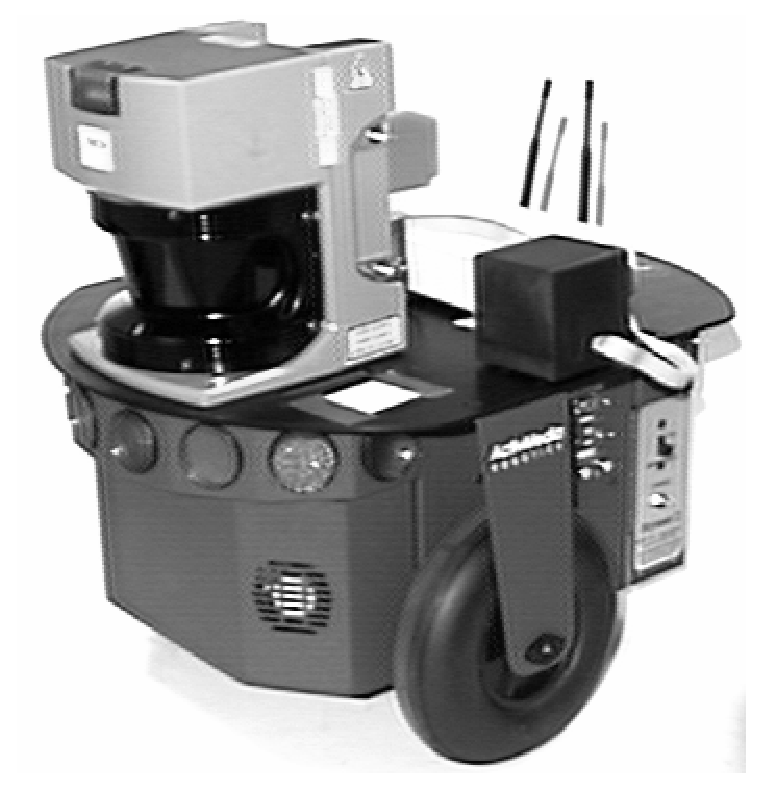
\epsfig{file=laser.eps,width=.75\columnwidth}
  \caption{{\sl Player can control many popular robot devices, including
                the Pioneer 2-DX mobile robot and peripherals pictured here.}  \label{fig:p2dx}}
\end{figure}
In order to provide a uniform abstraction for a variety of devices, we
chose to follow the UNIX model of treating devices as files.  Thus the
familiar file semantics hold for Player devices.  For example, to
begin receiving sensor readings, the client opens the appropriate
device with {\tt read} access; likewise, before controlling an
actuator, the client must open the appropriate device with {\tt write}
access.  In addition to the asynchronous data and command streams,
there is a request/reply mechanism, akin to {\tt ioctl()}, that
clients can use to get and set configuration information for Player
devices.  As this model has served UNIX-like operating systems well
for decades, we expect that it will be suitable for Player devices well
into the future.

Player does not implement any device locking, so when multiple clients are
connected to a Player server, they can simultaneously issue commands to
the same device.
In general, there is no queuing of commands, and each new command will
overwrite the old one.  We chose not to implement locking in order to
provide maximal power and flexibility to the client programs.  In our view,
if multiple clients are concurrently controlling a single device, such as a
robot's wheels, then those clients are probably cooperative, in which case
they should implement their own arbitration mechanism at a higher level than
Player.  If the clients are not cooperative, then the subject of research
is presumably the interaction of competitive agents, in which case device
locking would be a hindrance.

We have borrowed further from classic operating system design in the way
that we have separated device interfaces from device drivers.  For example,
in an operating system there is a joystick interface that defines the API for
interacting with joysticks, and there are joystick drivers that allow the
programmer to control various joysticks through that same API.  Similarly,
in Player, a device {\em interface} is a specification of data, command, and
configuration formats, and a device {\em driver} is a module that controls a
device and provides a standard interface to it.  

For example, probably the most commonly used Player interface is the
{\tt position} interface, which is used to control a mobile robot base.
This interface specifies a command format that includes velocity and/or
position targets and a data format that includes velocity and position status.
One implementation of the {\tt position} interface is Player's {\tt p2os}
driver, which controls research robots made by ActivMedia, including the
popular Pioneer 2-DX (Figure~\ref{fig:p2dx}).  Other drivers that control
other kinds of robots also support the {\tt position} interface, which
means that they all accept commands and return data in the same format.
In general, multiple drivers can support the same interface, and a driver
can support multiple interfaces.  We discuss some advantages of this design in
Section~\ref{sect:opp}.

\subsection{Stage goals and design}
\label{sect:stage}
\begin{figure}
  \centering
  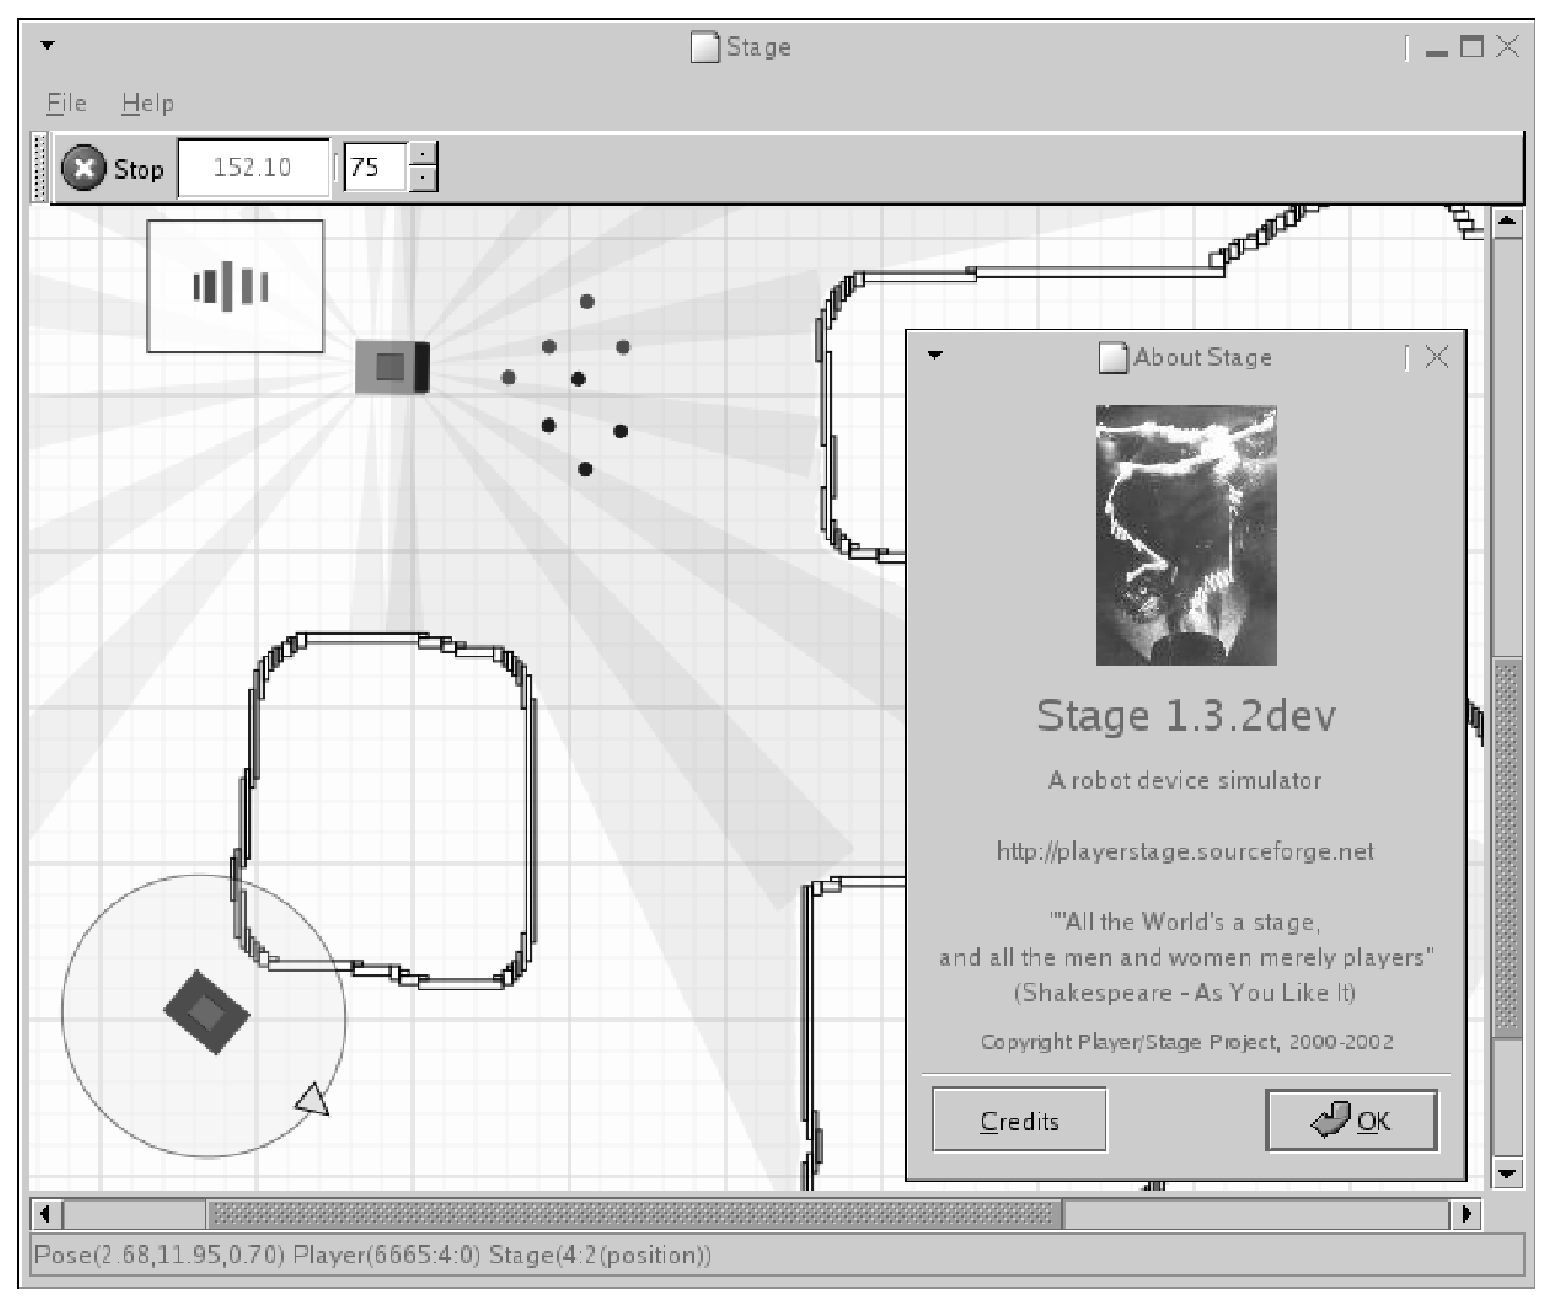
\epsfig{file=stage_screenshot_gray.eps,width=.9\columnwidth}
  \caption{{\sl Stage screenshot showing two robots (solid rectangles) with visualization of the top robot's laser range scanner, sonar and color blob-finder data. Stage's modular architecture allows multiple GUIs; this is GNOME2.}}
  \label{fig:screenshot}
\end{figure}


Stage simulates a population of mobile robots, sensors and
environmental objects. It has two original purposes; (i) to enable
rapid development of controllers that will eventually drive real
robots; and (ii) to enable robot experiments without access to the
real hardware and environments. In the last year or so, we have been
extending and generalizing the sensor models beyond the limits of any
available hardware, adding another purpose: (iii) to enable ``what
if?'' experiments with novel devices that do not (yet) exist.  This
path is developing with the help of DARPA, with the goal of using
Stage as a tool to determine the likely benefits of developing one
type of sensor over another. We return to this idea when discussing
opportunities for research, below.

Stage was specifically designed to support research into multi-robot
systems. When programming and experimenting with many robots the
benefits of rapid development are multiplied, and Stage enables
experiments with large populations of robots that would be
prohibitively expensive to buy and maintain. There are several aspects
of Stage's design that make it suitable for multi-robot systems:

\begin{itemize}
\item {\bf Good {\em enough} fidelity}: Stage provides fairly simple,
  computationally cheap models of lots of devices rather than
  attempting to emulate any device with great fidelity. Low fidelity
  simulation can actually be an advantage when designing robot
  controllers that must run on real robots, as it encourages the
  use of robust control techniques \cite{Jakobi:ab97}.  Low
  computational demands mean we can simulate many devices on commodity
  hardware.
  
\item {\bf Linear scaling with population:} All sensor models use
  algorithms that are independent of population size. Thus Stage's
  computational requirements grow linearly with
  population\footnote{Some future devices may not follow this rule, as
    some algorithms that scale as a power of the population size can
    be convenient to implement and will perform well with small
    populations.}.
  
\item {\bf Configurable, composable device models:} Various sensors
  and actuators are provided, including sonars, scanning laser
  rangefinders, visual color segmenters, fiducial detectors, and
  a versatile mobile robot base with odometry.  The models are often
  more general and flexible than any specific piece of hardware, so
  each model is configured to approximate the (real or imagined)
  target device. See the manual \cite{stagemanual} for a complete list
  of devices and their properties.
    
\item {\bf Player interface:} All sensor and actuator models are
  available through Player's standard interfaces. Typically, clients
  cannot tell the difference between the real robot devices and their
  simulated Stage equivalents (unless they try very hard).  Thus Stage
  inherits the flexibility of Player's non-locking, platform- and
  language-neutral interface for all its devices.

\end{itemize}

\subsubsection{Devices, populations and performance}
Devices can be composed in tree structures to build up complex robots.
For example, most users base their robots on the {\tt position} model
with a selection of sensor models on top. Several users \cite{HowardMataricSukhatme03,JungSukhatme02,MakarenkoWilliamsBourgault02,Vaughan02:LOST-tra}
have simulated the Pioneer 2DX pictured in Figure~\ref{fig:p2dx} with
a {\tt position} model carrying a {\tt sonar} array and {\tt laser}
scanning rangefinder. The Stage distribution includes some
commonly-used configurations, such as the geometry of the
Pioneer's sixteen sonar transducers.

By default, Stage attempts to run in real-time. Models are updated at
a fixed (configurable) interval.  If the update takes longer than the
suggested interval, simulations will run slower than real time. Device
models vary greatly in computational demands; the author's 600MHz Pentium
III Linux PC runs 200 sonar-guided robots ({\tt position} \& {\tt sonar}
models) or 15 laser-guided robots ({\tt position} \& {\tt
  laser} models) in real time at spatial and temporal resolutions of
  0.02m and 100ms, respectively.

In the optional ``fast mode'', Stage does not wait for the real-time
clock. Simple simulations will run much faster than real time,
which is useful for long or batch experiments (e.g., \cite{Dahl02}).
Time-sensitive clients use Player's internal clock to avoid time-warping
issues.

\subsubsection{Validity}
There is no guarantee that experiments in Stage are directly
comparable with those using real-world robots. However, users
have found that clients developed using Stage will work with
little or no modification with the real robots and vice versa
\cite{JungSukhatme02,MakarenkoWilliamsBourgault02,Vaughan02:LOST-tra}. As
the number of transfers between Stage and real robots increases,
users have an increasingly powerful argument to support the real-world
validity of Stage-only experiments.  This is a major advantage of using a
well-known simulator instead of home-grown, project-specific code.  Also,
Stage's Open Source license allows peer review of the simulation code,
and encourages sharing of models, configurations and environments.
Just as Player facilitates code re-use and sharing, Stage enables
experiment sharing. We hope to see standard test scenarios emerge, in
which users can compare their controllers. Already simulation experiments
are routinely carried out with one of Stage's example worlds, such as
``cave'' and ``hospital.''

\section{Opportunities for research}
\label{sect:opp}

Player makes it very easy for clients to read data from and send
commands to any device on the network, as well as send arbitrary
messages to one another. Stage allows for convenient and rapid
evaluation of many clients. Both programs constrain the design of
clients very little; they aim to provide transparent infrastructure
for MRS research. In this section we describe some of the research
opportunities enabled by the design decisions described above.

\subsection{Embedded systems}
The design of Player has been guided in part by our desire to maximize
its utility and applicability by keeping it small and fast.  Thus the
server core, which provides sophisticated client services, is actually
quite simple and has become more so over time as, for example, we have
collapsed most of its functionality into a single thread of execution.
The device driver system is modular, allowing the system designer to
include only those drivers that are necessary for a particular
application.\footnote{Without any device drivers, the Player server
  binary, as of version 1.3, is about 64KB.}  Because it is
small and fast, Player is equally well-suited to run on low-power
embedded systems and high-power workstations.  Player is currently
in use on embedded PPC/Linux and ARM/Linux systems.  As part of the
DARPA Software for Distributed Robotics (SDR) program, the first-ever
(to the authors' knowledge) 100-robot experiments will comprise a network
of such embedded computers, each running Player and controlling a small
mobile robot.

\subsection{Sophisticated devices}
\label{sect:soph-dev}
In addition to ``regular'' device drivers that provide an almost
transparent control interface to a piece of hardware, Player's
extensible device model allows sophisticated sensing and control
algorithms to be encapsulated in drivers.  These ``abstract'' drivers
can perform arbitrary computation, ranging from signal processing to
closed-loop control.  For example, Player includes both a {\tt
  waveaudio} driver that delivers raw audio data and a {\tt
  fixedtones} driver that performs a Fast Fourier Transform on the raw
data and reports the frequencies and amplitudes of the highest peaks
in the frequency domain.  Similarly, Player contains a collection of
{\tt fiducial} detectors, each designed to find a different kind of
landmark by processing data from various sensors.  One such detector
fuses information from a laser range-finder and a camera image and
incorporates control of a pan-tilt-zoom unit to find landmarks.
Recently, we have added drivers that implement different forms of the
widely-used Monte Carlo localization scheme.  When included as drivers
in the server, these algorithms become standard services that any
client can exploit, even without knowledge of how they work.

\subsection{Common device interfaces}
As mentioned in Section~\ref{sect:devmodel}, Player's device model
permits drivers that control different hardware or implement different
algorithms to present the same interface to the client.  As a result,
control programs can largely ignore the details of the underlying
hardware or algorithm, treating the system as a collection of generic
devices.  For example, the Player drivers that control mobile robot
bases made by ActivMedia, RWI, and K-Team all present the same {\tt
  position} interface.  Thus a Player client program can control any
of those robots, with little or no changes required to move between
platforms.  Several IMU drivers also present the {\tt position}
interface and so appear to be immobile bases.  Similarly, the landmark
detectors mentioned above all present the {\tt fiducial} interface,
so, for example, a client program that builds a landmark-based map can
employ the fiducials that are most appropriate to a given environment
but largely ignore which detector is in use.

\subsection{Novel sensing \& control systems}
As a result of its innovative network-centric architecture, Player
permits any client, located anywhere on the network, to access any
device; a robot can effectively ``see'' through its teammates' eyes.
Using Player as a substrate, novel distributed sensing and control
systems that were previously unrealizable can now be constructed quite
easily.  This feature was exploited in recent work on concurrent control
\cite{GerkeyMataricSukhatme02}, in which approximately fifty independent
agents were simultaneously controlling a single robot's motors through
Player.  Similarly, Player allowed a team of robots engaged in cooperative
localization \cite{HowardMataricSukhatme03} to directly access each
others' sensors, thereby facilitating sensor fusion.  In building such
systems, the designer is free to choose the most appropriate programming
language and computing platform to implement each component.

%README
A recent addition to the server is the ``passthrough'' driver.
Executing within the context of a Player server, this driver acts as a
client to another Player server.  The passthrough driver connects to a
remote server and provides a local proxy for a remote device by forwarding
commands and data.  In this way, remote resources can be made to appear as
local resources, which offers interesting avenues for future research.

%README
Consider the encapsulation of sophisticated algorithms into Player
drivers described in Section~\ref{sect:soph-dev}.  When algorithms are
made into drivers, they must run within Player on the server side,
which is often a robot.  If the robot has only modest computational
facilities, then it may not be well-suited to run, for example, an
expensive probabilistic localization algorithm.  In this case, another
instance of Player can run off-board, on a more powerful desktop machine,
with passthroughs providing data from and control of the remote devices.
An expensive algorithm can then run in the off-board instance of Player.
Using the passthrough driver, the computational load of a sensing and
control system can be distributed and arbitrarily located around a
network, so as to best exploit available resources.  Also, when working
with systems composed of many robots, a single instance of Player that
contains passthroughs for all of the robots' sensors and actuators can
act as a mechanism to aggregate data (e.g., for visualization or logging)
and/or distribute commands (e.g., for an operator console).

\subsection{Comparing controllers and performance metrics}
As a result of their flexibility and the Open Source development model,
both Player and Stage are becoming widely adopted. This provides the
potential for an open standard test platform which would encourage
objective evaluation and comparison of robot control algorithms. There
are currently very few practical metrics or other characterizations of
robot behavior, yet there is a lot of interest in this area. Such
evaluation will be required for the field to transition from a
primarily {\em ad hoc} experimental science to a more principled
discipline.

\subsection{Fantastic sensors}
Stage is normally used to simulate existing robot devices, as users
test the feasibility of their ideas for controlling real robots. But
Stage can be used as a ``what if'' tool, to explore robot controllers
that use devices that do not exist. This is useful as a conventional
design tool, allowing investigations such as: `How would my
localization algorithm perform with a device that performs half-way
between a sonar and a laser?', or `What are the trade-offs between
robot speed and battery life, or sensor update rates and resolution?',
`What novel algorithms could exploit an ultra-wide-band radar that
could detect walls {\it and} the objects behind them?'.  Robotics
projects that are developing a new sensor can experiment with
controllers in simulation before their hardware is ready.

Stage's modular architecture makes it easy to add entirely new models
in order to explore less common ground: 'What could I do if my robots
could change color at will, or visually express some internal states
to their colleagues, or quickly recognize and categorize each
other \cite{VaughanStoySukhatmeMataric00a}?'.  Exploring the use of devices
that are not currently feasible opens up a new field of study; robotics as
it {\it could be}. Freedom from practical constraints distinguishes science
from engineering; having a means to perform experiments distinguishes science
from science fiction.

\subsection{Challenges in scaling sensor-based simulation}
Stage simulates multiple devices and scales to a few hundred devices,
but is not currently useful for simulating massive populations, say on
the scale of an ant colony, which would be of great interest for MRS
researchers. It would be interesting to distribute Stage's compute
load over a cluster of computers to support very large populations
(tens of thousands) in real time. This is a significant technical
challenge that poses unsolved problems in representation and
synchronization. Stage would also benefit from advanced spatial
representation to improve speed and memory efficiency in large and/or
sparsely populated environments.

\section{Usage}
\label{sect:usage}
In 2002, software from the Player/Stage project was downloaded over 2000
times.  Player and Stage are currently in use in more than twenty major
academic and industrial research labs around the world, and are also used in
teaching undergraduate and graduate classes.  Given the modest size of the
target audience (i.e., robotics researchers and students), we consider the
project to be a significant success.  An important factor in that success
has been the Open Source model, which encourages inclusive, collaborative
software development.  As the developer team and user base have grown,
major enhancements have been made to the software.  Because of their modular
designs, Player and Stage are easily extended by, for example, encapsulating
a sophisticated control algorithm into the server or adding a model of an
unavailable but interesting sensor to the simulator.

Since it is the collective experience of the users that drives
development, we now briefly review a few projects in which Player and/or
Stage have been used.  One such project is concerned with robotic sensor
networks \cite{SibleyRahimiSukhatme02}, which are characterized by
extremely large collections of inexpensive mobile robots.  Given the
practical limitations on fielding even tens of physical robots, the
ability to simulate hundreds or thousands of robots in Stage is invaluable
to researchers wishing to test communication and coordination algorithms
on large-scale systems.  A similar project \cite{GrocholskyMakarenko03}
aims to extend the scalability and modularity of the Decentralized Data
Fusion (DDF) architecture to active sensor networks in which some or all
of the network components have actuators. The practical implementation
will be able to utilize the resources of a heterogeneous and dynamic team
of sensing platforms to find and track stationary and moving features in
an indoor environment.  Player is used as a common hardware abstraction
layer throughout the diverse set of software modules and Stage is used
extensively for code validation and initial performance assessment.

Another project \cite{JungSukhatme02} studies resource allocation
for target-tracking in sensor-actuator networks, using a region-based
approach to control deployment of mobile robots.  A multi-resolution
task assignment architecture allows the system to handle significant
environmental occlusion.  Because the same Player interface is used
with both physical and simulated devices, the tracking system that
was developed in Stage was trivially transitioned to real robots.
Resource allocation is also investigated from a learning perspective
\cite{Dahl02}, with the goal of developing general adaptive capabilities
in robots and multi-robot systems.  Focusing on spatio-temporal
adaptivity, this project uses reinforcement learning to allow robots
to dynamically adjust their behavior to any given environment while
performing a set task.  Of particular use in this project was Stage's
ability to run simulation trials faster than real time, and thereby
generate the substantial amount of data required to determine the run-time
characteristics and performance impact of the learning system.

Player is also used in an investigation of novel multi-robot task
allocation algorithms \cite{GerkeyMataric02b}, providing a unified
interface to a group of heterogeneous robots.  In this case,
an economically-inspired task auctioning system is developed and
validated on multi-robot teams, ranging in size from 3 to 7 robots,
engaged in a variety of tasks.  The resulting task allocation system,
{\scshape Murdoch}, is also used in a broader study of large-scale
human-system interaction \cite{TewsMataricSukhatme03}.  The coordination
infrastructure was originally developed and tested in Stage with a large
group of simulated robots and was then validated on a smaller team of
physical robots.  This simulate-validate approach has also been
successfully employed in many other projects, including recent work on
multi-robot resource transportation \cite{Vaughan02:LOST-tra}.

\section{Related work}
Lack of space precludes a detailed comparison of Player and Stage with
their alternatives; that is another paper. The distinguishing features of
tools developed by the Player/Stage project are (i) they seek to constrain
the design of the controlling client program as little as possible; and
(ii) they are efficiently implemented around a custom network server.

By minimizing constraints on the control program, Player and Stage offer a
uniquely flexible robot development environment compared to others such as
Saphira \cite{Konolige97}, Mission Lab \cite{MacKenzieArkinCameron97}, TeamBots
\cite{balch98}, Ayllu \cite{Werger00}, DCA \cite{PeterssonAustinChristensen01},
ARIA \cite{ARIA}, and CARMEN \cite{ThrunFoxBurgardDellaert01}.  As a tradeoff
for providing support for a particular control or coordination philosophy,
these systems all restrict the end-user's choice of programming language
and/or structure.  While such constraints can be very useful in guiding the
user in a particular paradigm, we believe that such low level constraints
are unsuitable for a general-purpose system; the programmer should have
the choice to build any kind of control system while still enjoying device
abstraction and encapsulation.  Thus in Player we make a clear distinction
between the {\sl programming interface} and the {\sl
  control structure}, opting for a highly general programming
interface, allowing users to develop their own tools, including sophisticated
architectures like those mentioned above.

Because it is designed explicitly for robotic device control, Player
is efficient for this purpose; the primary limitation on its
performance is currently the speed and fidelity and the underlying
operating system's scheduler.  By building a custom protocol and
server instead of adhering to a ``generic'' communications standard,
such as CORBA \cite{CORBA} or Jini \cite{Waldo99}, we are free from
the computational and programmatic overhead that is generally
associated with the practical application of such a standard.  Robot
interfaces that do rely on these standards, such as Mobility
\cite{mobility}, OROCOS \cite{orocos-web}, and others
\cite{BurchardFeddema96,Holness01}, benefit from readily-available
client-side libraries that hide many of the communication details.
However, as demonstrated by the proliferation of similar client-side
libraries for Player (currently available in 6 languages), our custom
message protocol is simple and easy to implement.

\section{Summary and future work}
\label{sect:conc}
The goal of the Player/Stage project is to provide Open Source software
infrastructure to support experimental research with multi-robot systems
(MRS).  To this end the project has developed the robot device server
Player and the multiple robot simulator Stage.  In addition to facilitating
ongoing MRS research, Player and Stage offer new opportunities for research
in emerging areas, including distributed sensing and control systems.
We expect these opportunities to improve and multiply as the software is
used and developed by more roboticists.

%README
Player and Stage are actively developed and we have numerous enhancements
planned for the near future.  Regarding Player, we plan to incorporate as
standard services more sensing and control algorithms, initially focusing
on enabling technologies such as localization and mapping.  To support
the construction and control of complex MRS, we are investigating methods
for resource discovery, as discussed in \cite{VaughanGerkeyHoward03}.
We will also add device drivers that support research with embedded
systems, including monitoring facilities for {\em ad hoc} networks and
sophisticated communication services.  In order to allow the simulation
of extremely large populations of such systems, Stage will soon be
distributible across networks of workstations or cluster computers.
One of our near-term goals is to deploy such a cluster as a public ``Stage
server'' that would simulate large worlds over long periods of time,
allowing the potential for comparison and evaluation of proposed control
algorithms in both cooperative and competitive settings.  Simultaneously,
we are improving Stage's performance by making the world representation
more efficient for sensor modeling.

%README
Finally, we are well advanced in the development of another
Open Source multi-robot simulator: Gazebo.  Whereas Stage is designed
to simulate very large numbers of robots in 2D indoor environments,
Gazebo is a full 3D dynamic simulation designed for the simulation of
small numbers of robots in outdoor environments.  Like Stage, Gazebo
is fully compatible with Player, and client programs can switch
between the two simulations without code modification.  An early
version of Gazebo should be available in August 2003.


\begin{Acknowledgment}
We thank the many developers and users who have contributed so much to the
success of the project, especially: 
Maxim Batalin,
Josh Bers,
Brendan Burns,
Jason Douglas,
Jakob Fredslund,
Kim Jinsuck,
Boyoon Jung,
Alex Makarenko,
Andy Martignoni III,
Nik Melchior,
Dave Naffin,
Esben \O{}sterg\aa{}rd,
Gabe Sibley,
Kasper St{\o}y,
John Sweeney 
and
Doug Vail.

%README
Thanks also to SourceForge.net for project hosting, and to Doug Gage
at DARPA IPTO for his valuable support. This work is supported in part
by DARPA grant DABT63-99-1-0015 (MARS) at USC and contract
N66001-99-C-8514 (SDR) at HRL.
\end{Acknowledgment}

\bibliographystyle{plain}
\renewcommand{\baselinestretch}{0}
{\small
\bibliography{player}
}

\end{document}

